\subsection{Componenti di una serie temporale}
In questa sottocapitolo ci soffermeremo a spiegare le componenti principali
che compongono una serie temporale per poterne analizzare l'andamento e/o
eventuali pattern ricorrenti sull'intera serie.


Molte volte è utile suddividere una serie temporale in più diverse componenti
distinte per poter analizzare singolarmente il loro comportamento e
riuscire ad inferire sul generale andamento della serie. Possiamo quindi
pensare ad una serie temporale come un insieme di 3 componenti principali:
Trend (andamento/tendenza), Stagionalità e Residui (più comunemente detta Noise).

\subsubsection{Trend}
La componente di trend è un pattern nei dati che mostra che mostra il 
movimento (andamento) di una serie verso valori relativamente più alti o più bassi 
in un lungo periodo di tempo. In altre parole, si osserva una tendenza quando 
la serie temporale presenta una pendenza crescente o decrescente. 
La tendenza di solito si verifica per un certo periodo di tempo 
e poi scompare, non si ripete. Ad esempio, una nuova canzone, 
che diventa di tendenza per un po' di tempo e poi scompare. 
Non c'è alcuna possibilità che torni in tendenza~\cite{gg:trend}.\\
Il trend potrebbe essere:
\begin{itemize}
    \setlength\itemsep{-0.6em}
    \item \textbf{Uptrend}: L'analisi delle serie temporali mostra un andamento generale al rialzo, quindi si tratta di Uptrend.
    \item \textbf{Downtrend}: L'analisi delle serie temporali mostra un andamento al ribasso, quindi si tratta di un downtrend.
    \item \textbf{Trend orizzontale o stazionario}: Se non si osserva alcun pattern, si parla di trend orizzontale o stazionario.
\end{itemize}

Nella pratica il trend viene calcolato utilizzando delle tecniche di smoothing come
\textit{moving average} (questo argomento verrà successivamente trattato in una sezione dedicata)
e quindi stimato.

\begin{esempio} [esempio pratico di trend]
    Consideriamo come serie temporale una serie la cui per ogni osservazione abbiamo
    la media mensile delle temperature della città di Beijing a partire 
    dal $01/01/2013$ al $01/01/2017$.

    \begin{figure}[H]
        \centering
        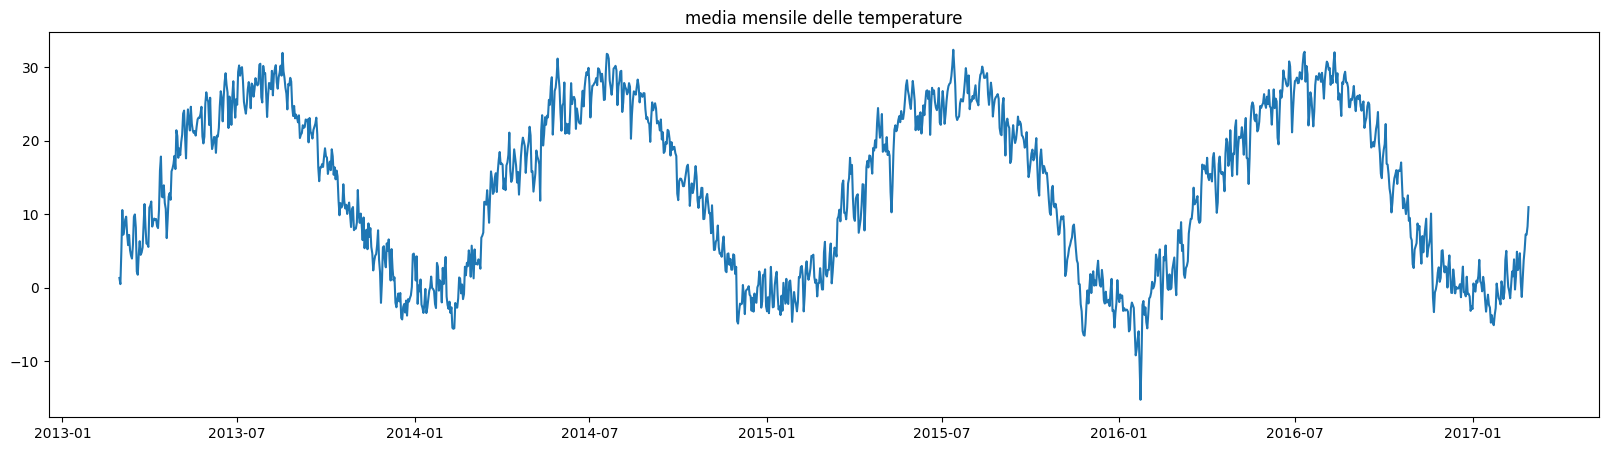
\includegraphics[width=\linewidth,height=4.7cm]{media_mensile_temp.png}
        \caption{Media mensile delle temperature della città di Beijing.}
    \end{figure}

    Consideriamo ora un periodo di un anno ($365$ giorni) il trend avrà un grafico
    come il seguente

    \begin{figure}[H]
        \centering
        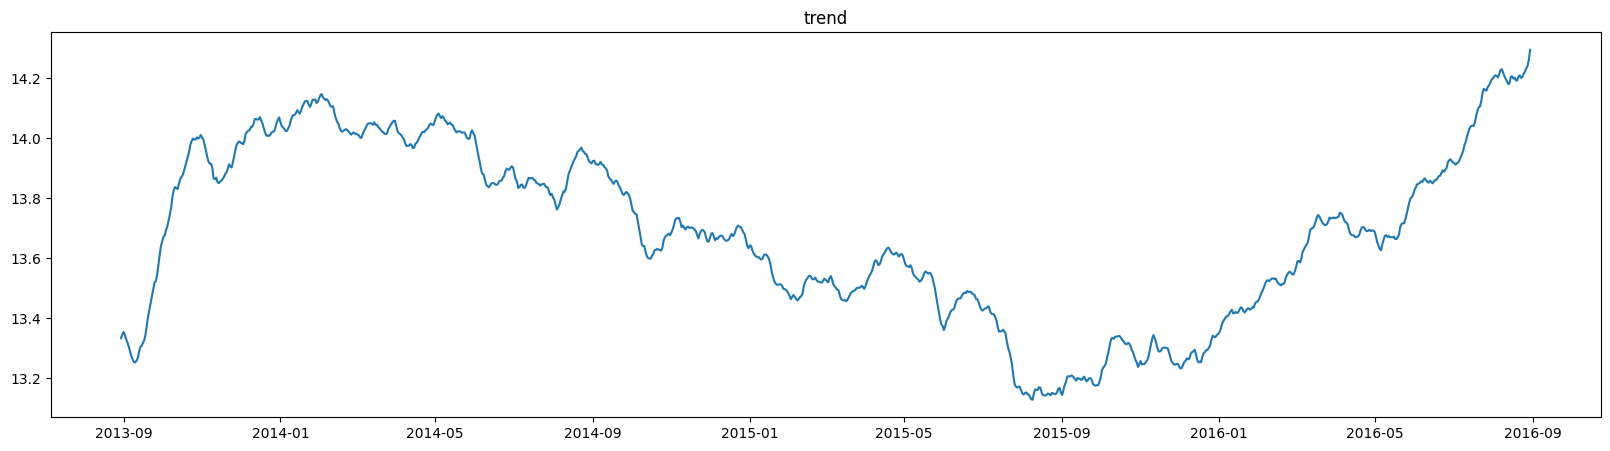
\includegraphics[width=\linewidth,height=4.7cm]{media_mensile_temp_trend.png}
        \caption{Trend media mensile delle temperature della città di Beijing.}
        \label{fig:media_mensile_temp_trend}
    \end{figure}

\end{esempio}


\subsubsection{Stagionalità}
La stagionalità è un aspetto cruciale dell'analisi delle serie temporali. 
Poiché le serie temporali sono indicizzate in avanti nel tempo, sono soggette a 
fluttuazioni stagionali. Ad esempio, ci aspettiamo che le vendite di gelati siano 
maggiori nei mesi estivi e minori in quelli invernali.

La stagionalità può manifestarsi in diversi intervalli di tempo, 
come giorni, settimane o mesi. La chiave per l'analisi delle serie temporali 
è capire come la stagionalità influisce sulle nostre serie~\cite{md:seasonality}.


\subsubsection{Residui}



\subsubsection{Decomposizione di una serie}
Esistono due modalità distinte per la decomposizione di
una serie temporale nelle sue 3 componenti principali. La prima modalità è detta
additiva in cui le componenti vengono semplicemente sommate, mentre la seconda
è detta moltiplicativa dove le componenti, come suggerisce il termine, 
vengono moltiplicate.

\paragraph{Decomposizione additiva} 
Una decomposizione additiva consiste nella
somma delle componenti. Se consideriamo una serie temporale ad un 
istante $t$ allora essa sarà composta da
\[ y_t = S_t + T_t + R_t \]
dove $y_t$ è l'osservazione, $S_t$ è la componente di stagionalità, 
$T_t$ è la componente di Trend ed $R_t$ è la componente dei residui, tutti
all'istante di tempo $t$.
\begin{figure}[H]
    \centering
    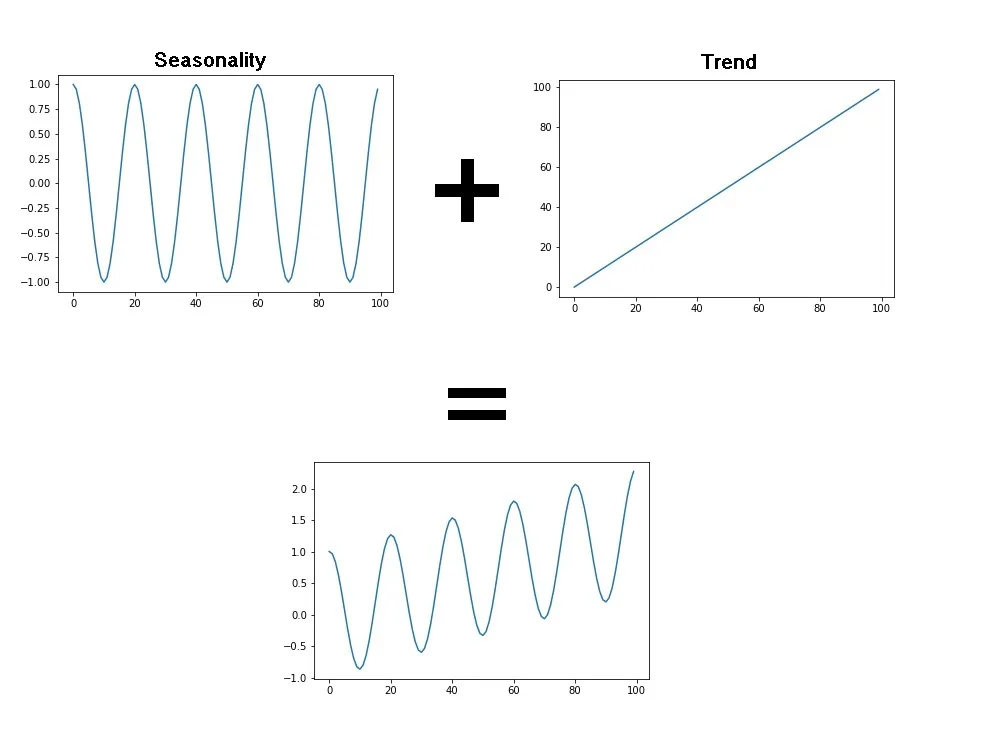
\includegraphics[width=0.6\linewidth]{additive_decomposition.jpg}
    \caption{Decomposizione additiva (escluso residui).}
\end{figure}


\paragraph{Decomposizione moltiplicativa} 
Una decomposizione moltiplicativa consiste nella
moltiplicazione delle componenti. Se consideriamo una serie temporale ad un 
istante $t$ allora essa sarà composta da
\[ y_t = S_t \times T_t \times R_t \]
dove $y_t$ è l'osservazione, $S_t$ è la componente di stagionalità, 
$T_t$ è la componente di Trend ed $R_t$ è la componente dei residui, tutti
all'istante di tempo $t$.
\begin{figure}[H]
    \centering
    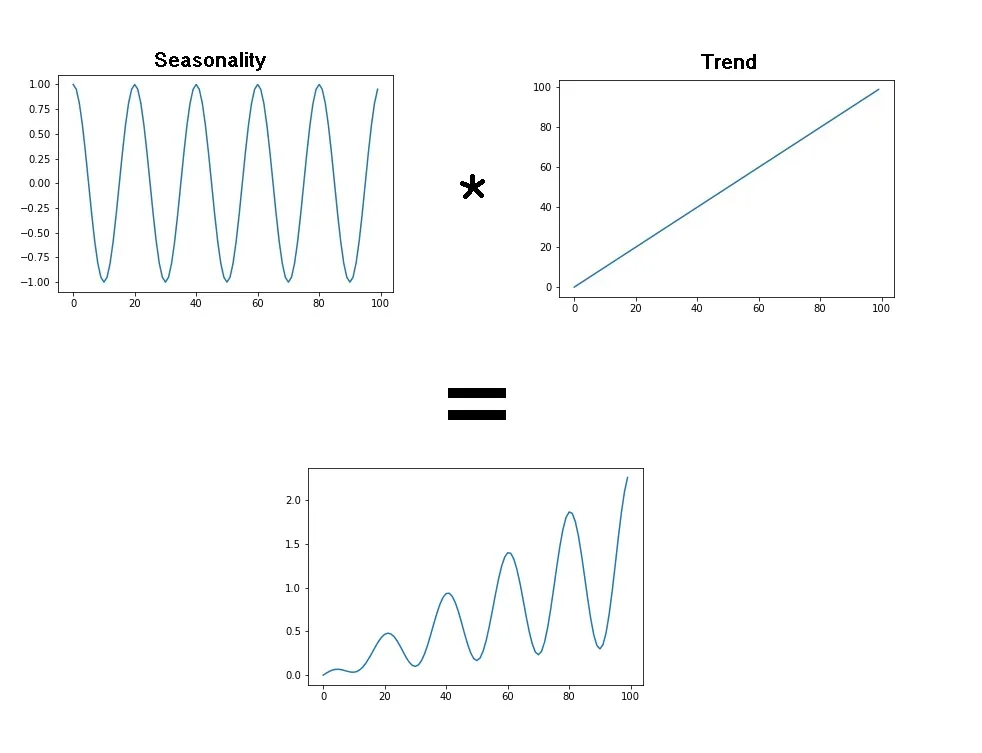
\includegraphics[width=0.6\linewidth]{multiplicative_decomposition.jpg}
    \caption{Decomposizione moltiplicativa (escluso residui).}
\end{figure}

\paragraph{Scelta della modalità di decomposizione}
La sceltà della modalità di decomposizione di una serie temporale è importate poichè
la sua decomposizione potrebbe apparire insensata scelta la modalità sbagliata.
Una decomposizione additiva è principalmente appropriata se il magnitudo della 
stagionalità non varia con il livello della serie temporale mentre se, la variazione
della componente di stagionalità, appare proporzionale al livello della serie una modalità
moltiplicativa potrebbe essere più appropriata.




